\chapter{Introduction}\label{c:i}
%
\section{Computational Methods in Chemistry}
%
Computantional chemistry enables the study of chemical systems in ways that traditional techinques cannot \cite{book1}. For example, solvent effects in chemical reactions \cite{ap1} without carrying out the reaction under different solvents and isolating intermediaries. Computational chemistry can also be very valuable for the pharmaceutical industry \cite{pharm7}; particularly the area of cheminformatics, which can greatly speed up the search and sorting of potentially bioactive molecules \cite{pharm2,pharm3}. For example, the discovery DNA gyrase inhibitors with higher affinity than previously known ones \cite{pharm4,pharm5,pharm6}. These techniques are usually extremely fast, for instance, in 2001 a laptop with a 3 GHz processor estimated the ADME \cite{inf} physical properties of 71,500 compounds in 3 minutes using the QikProp package \cite{pharm1}, providing relevant information for further study.

Nowadays, computational chemistry has permeated popular culture in the form of Folding@Home and the Clean Energy Project. Folding@Home currently outputs $48,000$ teraflops of computing power ($ 48,000 \times 10^{12}$ floating point operations per second). F@H focuses on the study of misfolded proteins in Alzheimer's, Huntington's, ALS, Mad Cow, Parkinson's, many cancers, among others \cite{f@h}. On the other hand, the Clean Energy Project focuses on the search and analysis of possible candidates for use in renewable energy projects, and had a cumulative total of 22,564 CPU years up to Jan 17 2014 \cite{cep}.

However, behind the broad range of applications, lie the theory and algorithms which make it all possible. Utilising theoretical techniques and efficient algorithms one can calculate, observe, and explore some of the most fundamental characteristics of chemical systems. Namely: vibrational modes, intermolecular interactions, and electronic structure, all of which can be analysed independently and on different levels of detail \cite{book2}; though sometimes, the problem requires some degree of interdependency.

Computational methods typically fall into four groups \cite{md1,gromacs}:
\begin{inparaenum} [1)\upshape]
	\item \emph{Ab initio} methods start from physical constants and are purely quantum-mechanical, dealing with all the problems N-body interacting systems bring.
	\item Molecular Dynamics (MD) methods apply classical mechanics to chemical systems. They are typically used in the analysis of large-scale systems, where other methods would take too long 	for a small increase in overall accuracy.
	\item Semi-empirical methods use experimental parameters as well as \textit{ab initio} techniques, sacrificing accuracy in the name of speed.
	\item Density Functional Theory (DFT) methods are often mentioned as a subset of \emph{ab initio} methods. DFT methods create a spatially dependent electron density function, reducing the 	problem from N electrons with 3N spacial dimensions to 3 spatial dimensions. Thus greatly reducing computational time. The caveat is that DFT methods are not suitable for strongly correlated 	systems. They can be extended to accomodate time dependency, such methods are called TD-DFT.
\end{inparaenum}

Which method is best suited for one's needs depends on the complexity of the system to be studied, the desired accuracy, and available computational resources \cite{molcas2}. Purely quantum mechanical methods such as \emph{ab initio} and DFT are particularly afflicted by scaling\footnote{\label{fn:1}Scaling is represented by asymptotic notation, $O(f(x))$ \cite{perturbation}, which summarises the computational time dependence as a function of the number of objects to analyse. However, only the function's dominant term is represented \cite{bigo}. For example: $ O(N^{M}) $ means polynomial scaling of order $ M $ \cite{poly_scale}; $O(N!) $ stands for factorial scaling \cite{fact_scale}; $O(C^{N})$ represents exponential scaling \cite{exp_scale}; and $O(M\log(N)) $ logarithmic scaling \cite{log_scale}.} issues \cite{scale}. \Cref{t:scale} shows scaling as a function of the number of atoms and basis set size in the calculation of Coulombic repulsion in two DFT methods \cite{qchem}.

\begin{table}
	\begin{center}
		\caption[Scaling differences in the calculation of Coulombic repulsion in two DFT methods.]{Scaling differences in the calculation$ ^{*} $ of Coulombic repulsion in two DFT methods (times in minutes). The calculations were carried out on alanine oligomers of 5, 10 and 15 amino acids. Scaling as a function of basis set went from $ O(N^{4}) $ to $ O(N^{2}) $ with the new method. Table edited from \cite{qchem}.}\label{t:scale}
	    \begin{tabular}{lcccccc}
    		\hline\\[-4mm]
	    	Basis Set$ ^{\dag} $ & 5(old) & 5(new) & 10(old) & 10(new) & 15(old) & 15(new) \\
		    \hline\\[-4mm]
    		6-31G(df,pd) & 39    & 27    & 145   & 98    & 263   & 169 \\
	    	6-31G+(df,pd) & 109   & 46    & 736   & 160   & 1240  & 362 \\
		    cc-pvdz & 56    & 20    & 177   & 79    & 369   & 143 \\
    		cc-pvtz & 361   & 85    & 1165  & 280   & 2482  & 551 \\
	    	\hline\\[-4mm]
	    \end{tabular}
    \end{center}
    {\footnotesize $ * $ Calculations carried out on a single 2 GHz processor of an Opteron cluster.\\
	$ \dag $ Basis sets in the form of $ X-YZ $G mean that internal orbitals are composed of $ X $ Gaussian primitives (G), while valence orbitals are composed of two functions each; the first is composed of a linear combination of $ Y $ G; the second of a linear combination of $ Z $ G. The + sign indicates the use of diffuse functions, and the parentheses the use of polarisation functions composed of a linear combination of orbital type $ p,~d,~f $ functions as the case may be. Basis sets of the type cc-pv$ n $z where $ n = $ d, t, q$,~ 5,~ 6 \dots $ where (d = double, t = triple, q = quadruple) contain correlation-consistent polarisation functions for valence orbitals; cc-p means `correlation-consistent polarised' and `v' indicates that they only model valence orbitals \cite{book2,basisset1,basisset2}.}
\end{table}

If the algorithms used are perfect, an increase in speed necessarily means a decrease in accuracy---an increase in speed would require the use of mathematical (truncated series, averages, symmetries) and/or physical (locality constraints, potential wells, classical mechanics) shortcuts, as well as the experimental parameters---by simplifying the problem and reducing the total number of operations required \cite{molcas1}. For this reason, the creation of new methods, models and algorithms is of the utmost importance (see \cref{t:scale}). In fact, computational time restrictions are the main reason why semi-empirical and MD methods are widely used in chemical biology and pharmacology \cite{md2,pharm}.

As previously mentioned, molecular dynamics applies classical mechanics to molecular systems. In other words, they apply classical-mechanical principles to systems which require quantum mechanical ones, leading to incomplete and erroneous descriptions \cite{moldyn}. Cases whose scale prohibits a purely quantum treatment, but also require accurate analyses, are analysed with semi-empirical and hybrid models which can extract quantum information (often of semi-quantitative accuracy) from MD simulations. This motivated the creation of the original ``quasiclassical'' model \cite{QC1}, which has traditionally been the easiest way to extract quantum information from MD simulations. It has often (but not always) been of semi-quantitative accuracy, motivating Meyer and Miller to modify and improve it \cite{cmsym}. With said modifications, the Meyer-Miller model (MM), was successfully applied to three non-adiabatic electronic processes originally defined by Tully and a few problems which use the spin-boson model \cite{tully,project}.
%
\section{Meyer-Miller Quasiclassical Trajectory Model with Symmetrical Windowing for Quantum States}\label{s:model}
%
The current iteration of Meyer and Miller's Quasiclassical Nuclear Trajectory Model (MM model) has been tested on four problems: simple avoided crossing, double avoided crossing, extended coupling and the spin-boson model for non-adiabatic dynamics of condensed-phase matter \cite{project}. For the sake of brevity and relevance in \cref{c:i}, it will only be explained in broad terms, a more detailed discussion can be found in \cref{c:mm}.
%
\subsection{Qualitative Description of the Model}\label{sb:qdm}
%
\Cref{c:mm} provides a detailed mathematical description of the model and its modifications, for \cref{c:i} it is enough to describe the general algorithm.
\begin{enumerate}
\item Assign initial positions and states of all atoms involved.
\item Assign initial momentum and action-angle variables of all atoms involved. The initial momentum must be in the direction of the target atom(s).
\item Calculate the initial state window function.
\item Evolve the trajectories with a numerical integration routine. The integration range is defined by the user/problem.
\item Calculate the final state according to the selection criteria.
\item Calculate the final state window function.
\item Save the final state window function for later use in Monte-Carlo averaging.
\item Repeat the process a statistically sensible number of times.
\item Average the initial and final state window functions.
\item Calculate the probability of every event.
\end{enumerate}
%
\section{Proposal}\label{s:p}
%
In order to explore the workings and robustness of the MM model, it will be applied to the analysis of the of four model systems. The model will be implemented in \textsc{fortran 2008} and will eventually be incorporated into the non-commercial computational and quantum chemistry package \textsc{cfour} \cite{cfour}, primarily developed by the Stanton and Gauß research groups. It will be validated by reproducing the results obtained by Meyer and Miller \cite{project}, and used to carry out calculations for different initial states and different conditions for the spin-boson model.

The code will also be generalised as much as possible so it can eventually be added to \textsc{cfour} \cite{cfour}.
%
\subsection{Broad Methodology}
%
The following list of actions is the methodology with which the problem will be tackled.
\begin{enumerate}
\item Obtain equations of motion.
\item Write pseudo-code (list of actions). This is similar to the description given in \cref{sb:qdm} but slightly more detailed.
\item Translate pseudo-code to \textsc{fortran 2008}. This version of \textsc{fortran} was chosen due to its relative ease of use, speed and ample parallelisation potential.
\item Characterise the code.
\item Validate the code by reproducing Cotton and Miller's results \cite{project}.
\item Obtain new results.
\item Generalise the code as much as possible.
\end{enumerate}
%
\section{Conclusions}\label{s:ic}
%
The model has been proven to be of qualitative and quantitative accuracy for the problems defined by Tully \cite{tully,project}, and will be used to generate new results for variations of these systems.

It's worth repeating that the development of different ways of doing things is always worth a fair try. It is why one of the objectives of the present thesis is to sufficiently generalise it so it can eventually be placed at the disposition of the scientific community by including it in \textsc{cfour}.

In all, computational chemistry is a large toolbox with which we can analyse a wide range of phenomena, which would otherwise be inaccessible---or at least---extremely difficult for us to study. And thanks to the wide variety of chemical systems, there is always need to expand it. However, this is \emph{not} the only motivator. The same drivers that haunt and propel all of mankind's endeavours: money, time, ego, efficiency and sheer curiosity; also apply to computational chemistry. For all these reasons, the search for different ways of doing things is of the utmost importance. In a sense, whether these methods work or not, is irrelevant. The fact that they exist and can be used, modified and studied, makes them invaluable for science, as they offer bifurcations in the road to a goal; bifurcations which may lead elsewhere interesting, or---at the very least---provide a different looking-glass through which to see the problem at hand.
\begin{comment}
%
Nature is full of phenomena that according to our intuition and knowledge, should be simple to comprehend, analyse and explain; however closer inspection often reveals the problem to be much more than first impressions let on. Such is the case of the vibronic structure of the \ce{NO3} radical.

The problem has been extensively analised by Stanton, utilising quantum-mechanical methods \cite{no3radical,no3radical1,no3radical2,no3radical3}. Nevertheless, there exists no comprehensive description of it. Which calls for the use of different methodologies in an attempt to do so. Furthermore, the development and/or utilisation of different methods in the analysis of the same problem not only aids in its resolution, but also serves to expand the toolbox known as computational chemistry. The selfsame technique often results in the generalisation, validation, improvement and even development of new methods \cite{tf}.

In order to better illustrate the problem, I ran calculations using \textsc{orca} \cite{orca}, shown later in Chapter \ref{c:i}.

\section{NO$_{3}$}\label{s:no3}

It is generally accepted that \ce{NO3} possesses a planar almost equilateral triangular equilibrium geometry; according to computational and experimental evidence, it presents a slight $ \mathbf{D_{3h}} \rightarrow \mathbf{C_{2v}} $ deformation \cite{no3radical1}.

\subsection{Role of NO$_{3}$ in Atmospheric Chemistry}\label{sb:atm}

\begin{figure}[t]
	\centering
	\includegraphics[width=\textwidth]{atm.eps}
	\caption[Role of \ce{NO3} in the Atmosphere.]{Role of \ce{NO3} in the Atmosphere. Diagram obtained from \cite{no3origin}.}\label{no3atm}
\end{figure}
\ce{NO3} plays an important part in atmospheric chemistry as shown in \ref{no3atm}. It is an integral part of the nitrogen, carbon and ozone cycles. Such a wide influence makes it of particular importance to life on earth---which would simply be impossible to maintain in its current form if any cycle were to be severely disturbed.

\ce{NO3} is generated from ozonolisis of nitric oxides. The reaction predominantly occurs at night because UV light catalyses the inverse reactions. It plays an important role in vegetated areas---where it oxidises and nitrates terpenes, isoprenes and alquenes emitted by vegetation; oceanic regions---where it reacts with dimethyl sulphoxide released by phitoplankton; and urban environments---where it reacts with nitrogen oxides emitted by human activity \cite{no3origin}.

\section{Vibrational Modes}\label{s:vm}

In order to properly define vibronic structure we must first understand vibrational modes. These are the relative movements of one or more atoms with respect with the rest. They are a direct consequence of the Heisenberg uncertainty principle, which states that the more one knows of a particle's momentum, the less one knows of its position $ \sigma_x \sigma_p \leq \frac{\hbar}{2}$, where $ \sigma = \text{standard deviation} $, $ x = \text{position} $, $ p = \text{momentum} $ and $ \hbar = \frac{h}{2 \pi} $ known as the reduced planck constant. The uncertainty principle is a direct consequence of the wave-like nature of quantum particles. In simpler terms, in order to know the precise momentum of a wave, one has to look at a large space; in doing so, one looses information on the particle's precise position. Likewise, if we only look at a small space we can acquire precise information of the particle's position, but not its momentum. The mathematical reason for this is that a wave's momentum ($ p $) is related to its frequency (it is the Fourier transform from the position domain into the frequency domain) and for wave-like particles, this frequency ($ \nu $) is related to the de Broglie wavelength ($ \lambda $) by $ p = \frac{h}{\lambda} = \frac{E}{c} = \frac{h \nu}{c}$ where $ E = \text{energy} $ and $ c = \text{speed of light} $.

The number of vibrational modes in a non-linear molecule is $ 3N-6 $, where $ N $ is the number of atoms. The formula is derived from observing that each atom has 3 degrees of liberty $ (x,y,z) $, from where $ 3N $ comes from. But there exist a number of linear combinations of movements which keep the molecular geometry unchanged (the relative position of all atoms remains unchanged), but change their absolute position. These include: movements along three axes, and rotations about them---giving a total of 6 degrees of movement which preserve molecular geometry. For linear molecules the number of modes is $ 3N-5 $ because rotations about the main axis do not change a molecule's geometry. The specific shape of each movement depends on the molecule's symmetry group.

Vibrational modes can be experimentally observed through the use of Raman and Infrared (IR) spectroscopy. Raman-active modes are those which modify the molecule's polarisability , while infrared active modes are those which modify its dipole moment\footnote[2]{S. Thomas, ``Infrared and Raman Spectroscopy''. \url{http://serc.carleton.edu/NAGTWorkshops/mineralogy/mineral\_physics/raman\_ir.html}}. The frequency (IR) or shift (Raman) at which modes are observed, depend on the atoms and bond types involved. For our present purposes, we are only interested in IR-active modes.

\subsection{Infrared Spectroscopy}\label{sb:ir}

The main problem presented by \ce{NO3} is that its vibrational modes do not correspond to the experimental evidence. Its IR spectrum is much more complex than it should (see Table \ref{t:spec1}). However, before going into further detail, it would be useful to understand an simple example. Figure \ref{f:form} showcases two spectra of formaldehyde, one simulated and another experimental.

\begin{figure}[t]
	\centering
	%\resizebox{1.0\textwidth}{!}{\input{irform}}
	\includegraphics[scale = 0.5]{irform.eps}
	\caption[Simulated and experimental IR spectra of formaldehyde.]{Simulated (solid red line) and gas-phase experimental (dotted blue line) IR spectra of formaldehyde. Simulated spectrum calculated with \textsc{orca} using \textsc{sto-6311g** dft/b3lyp} \cite{orca}. Data for the experimental spectrum obtained from \cite{formgasir}.}
	\label{f:form}
\end{figure}
In this kind of spectroscopy, organic molecules' bonds' vibrational energy and the incident photon's energy are approximately 1 order of magnitud from one another. Furthermore, it requires the presence of a permanent or induced dipole moment (dipole moment different to zero\footnote[3]{$ \mathbf{p(r)} = \sum\limits_{i=1}^{N} q_{i} (\mathbf{r}_{i} - \mathbf{r}) \neq 0$, where $ q_{i} $ is the charge $ i $ and $ \mathbf{r}_{i} $ its position with respect to the observation point $ \mathbf{r} $ (commonly the centre of mass).}) which changes during the vibration. This type of spectroscopy is classified as absorptive, given that the photon's energy is absorbed by the by the bond, and its energy transferred into the vibrational process.

The discrepancies seen in Figure \ref{f:form} are due to various reasons. Two of which can be traced to the number of molecules involved in either case. In simulation, one analyses an isolated molecule, which is why all peaks are clearly defined. Experimentally, that is impossible, so there are bound to be interactions between the involved molecules. Aggravatingly (in this case), if there is trace water--very likely considering it's formaldehyde--condensation reactions can occur, leading to the formation of a variety of oligomers. These interactions and reactions complicate the spectrum, broadening, intensifying, dampening and even creating new peaks. The third reason as to why experimental and simulated spectra differ is vibronic structure, which will be simply explained in \ref{sb:vib}.

\subsection{IR Spectrum of NO$ _{3} $}\label{sb:irno3}

Table \ref{t:spec1} shows the experimental and simulated IR spectra of \ce{NO3}, as well as their band assignations and vibrational classification. Figure \ref{f:irteono3} shows a simulated \ce{NO3} IR spectrum.s:ic
\begin{table}
	\centering
	\caption[Experimental and simulated IR spectrum and frequency assignation of \ce{NO3}.]{Experimental and simulated IR spectrum and frequency assignation of \ce{NO3}. Where $ \nu_{1} $ is a totally symmetric N--O stretching; $ \nu_{2} $ an out-of-plane bending; $ \nu_{3} $ a degenerate N--O stretching; and $ \nu_{4} $ a degenerate in-plane bending. $ \updownarrow $ denotes parallel bands and $ \leftrightarrow $ perpendicular ones \setcounter{footnote}{3}\protect\footnotemark. Table edited from \cite{no3radspec}.}
	\label{t:spec1}
	\begin{subtable}{\textwidth}
		\centering
		\caption{Experimental vibrational modes of \ce{NO3}.}\label{t:exp}
    	\begin{tabular}{rccl}
        	\hline\\[-4mm]
	    	Band & $I$ & \multirow{2}[2]{*}{Type} & Vibrational \\
    		(cm\textsuperscript{-1}) & (Relative) &       & Assignment \\
        	\hline\\[-4mm]
	    	759   & 0.3   & $\updownarrow$ & $\nu_{2}+\nu_{4}-\nu_{4}$ \\
    	    762   & 0.8   & $\updownarrow$ & $\nu_{2}$  \\
    		1492  & 4.7   & $\leftrightarrow$ & $\nu_{3}$ \\
	    	1927  & 3.0   & $\leftrightarrow$ & ?      \\
    		2024  & 1.5   & $\leftrightarrow$ & $5\nu_{4}$  \\
    		2155  & 2.0   & $\leftrightarrow$ & $\nu_{1}+3\nu_{4}$  \\
	    	2200  & 0.7   & $\leftrightarrow$ & ?    \\
    	    2240  & 0.4   & $\leftrightarrow$ & ?      \\
    		2380  & 0.4   & $\leftrightarrow$ & ?     \\
	        2518  & 2.1   & $\leftrightarrow$ & $\nu_{1}+\nu_{3}$ \\s:ic
    		2585  & 1.7   & $\leftrightarrow$ & $2\nu_{1}+3\nu_{4}$ \\
    		7602  & 0.14  & $\updownarrow$ & $\nu_{4}$ \\
	        7744  & 0.4   & $\leftrightarrow$ & $\nu_{2}$   \\
    	    \hline\\[-4mm]
        \end{tabular}
	\end{subtable}
	\\[0.5cm]
	\begin{subtable}{\textwidth}
		\centering
		\caption{Vibrational modes calculated using \textsc{orca} with \textsc{sto-6311g** dft/b3lyp} \cite{orca}.}
    	\begin{tabular}{cccc}
		    \hline\\[-4mm]
			Band & $I$ & \multirow{2}[2]{*}{Type} & Vibrational \\
			(cm\textsuperscript{-1}) & (Relative) &       & Assignment \\
			\hline\\[-4mm]
			$ 259 $   & $ 0.898 $ & $ \leftrightarrow $ & $ \nu_{4} $\\
			$ 293 $   & $ 1 $ & $ \leftrightarrow $ & $ \nu_{4'} $\\
			$ 801 $   & $ 0.898 $ & $ \updownarrow $ & $ \nu_{2} $\\s:ic
			$ 1118 $ & $ 0.005 $ & $ \leftrightarrow $ & $ \nu_{3} $\\
			$ 1133 $  & $4 \times 10^{-4}$ & $ \leftrightarrow $ & $ \nu_{1} $\\
		\hline\\[-4mm]
		\end{tabular}\\
	\end{subtable}
\end{table}

\begin{figure}[t]
	\centering
	%\resizebox{1.0\textwidth}{!}{\input{irtno3}}
	\includegraphics[scale=0.5]{irtno3.eps}
	\caption[Simulated IR spectrum of \ce{NO3}.]{Simulated IR spectrum of \ce{NO3}. Calculated using \textsc{orca} with \textsc{sto-6311g** dft/b3lyp} \cite{orca}.}
	\label{f:irteono3}
\end{figure}

It is evident from Table \ref{t:spec1} that there exists no significant correlation between simulation and experiment. The only band which is relatively in close in all categories is an out-of plane bending parallel band that appears at 801 and 762 cm\textsuperscript{-1} in the simulated and experimental spectra respectively. Additionally, the simulations erroneously indicate the existence of a single degenerate mode, $ \nu_{3} $, when in reality there are two, $ \nu_{3} $ and $ \nu_{4} $ \cite{no3radspec}. These discrepancies are too large to be solely attributed to intermolecular interactions, which broaden and displace peaks, but preserve the general spectral structure, just as in Figure \ref{f:form}. In this case, however, both spectra are completely different.

\footnotetext{\label{fn:3}A band is classified as perpendicular if the change in the dipole moment is perpendicular to its major rotational axis. Likewise, it is classified as parallel when the change is perpendicular to the major rotational axis.}
\subsection{Vibronic $ \equiv $ Vibrational $ \oplus $ Electronic}\label{sb:vib}

The concept of vibronic structure deals with the relationship between vibrational and electronic states. Figure \ref{f:vibronic} is a simple, fictitious diagram that illustrates the concept.
\begin{figure}[t]
	\centering
	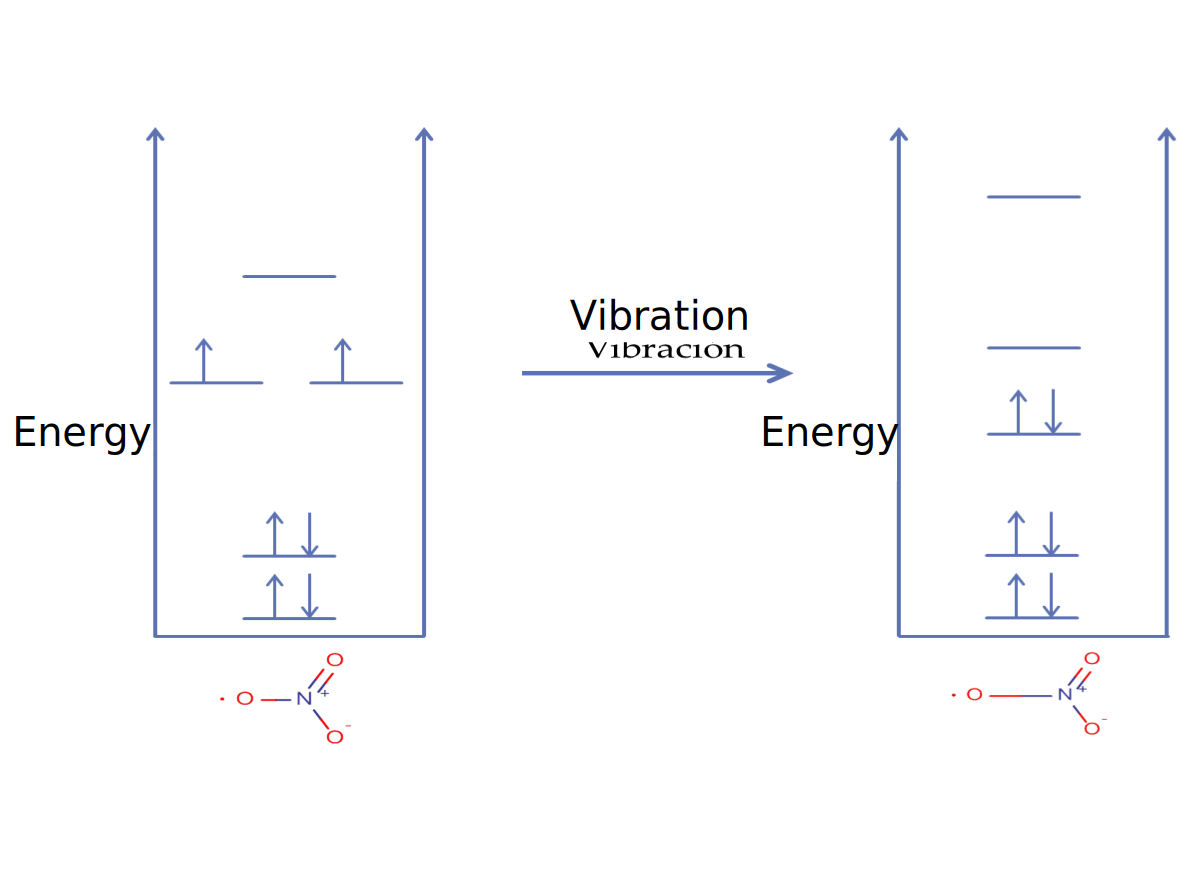
\includegraphics[width=\textwidth]{vibronic.eps}
	\caption[Diagram of a fictitious vibronic structure.]{Diagram of a fictitious vibronic structure. Horizontal bars indicate electronic states, arrows indicate electrons and their spin.}
	\label{f:vibronic}
\end{figure}
Initially, a molecule finds itself in its equilibrium geometry. Suddenly, one of the bonds absorbs a photon, whose energy is transferred into the bond as a vibration which changes the molecule's geometry (and possibly symmetry), consequently so do the shapes and energies of its molecular orbitals (MOs). In the diagram, both degenerate orbitals (orbitals with the same energy) change their energies, and so does the molecule's multiplicity. These relatively drastic changes of energy, multiplicity and symmetry open the floodgates to a myriad of previously inaccessible vibrational modes. To compound the issue, the process can repeat itself indefinitely, giving rise to the final jumble of vibrational modes observed experimentally in Table \ref{t:spec1}.

This problem has been extensively researched from a purely quantum-mechanical perspective by Stanton \cite{no3radical,no3radical1,no3radical2,no3radical3}. However, this type of analysis is extremely complicated and laborious, as it entails carrying out time-dependent calculations of simultaneous, interacting processes. For this reason, it is important to explore other avenues of analysis.

\section{Quasiclassical Nuclear Trajectory Model}\label{s:model}

The current iteration of Meyer and Miller's quasiclassical nuclear trajectory model (MM model) has been tested on four problems: simple avoided crossing, double avoided crossing, extended coupling and the spin-boson model for non-adiabatic dynamics of condensed-phase matter \cite{project}. For the sake of brevity and relevance in Chapter \ref{c:i}, it will only be explained in broad terms, a more detailed discussion can be found in Chapter \ref{c:mm}.

\subsection{Qualitative Description of the Model}\label{sb:qdm}

Chapter \ref{c:mm} provides a detailed mathematical description of the model and its modifications, for Chapter \ref{c:i} it is enough to describe the general algorithm.
\begin{enumerate}
\item Assign initial positions and states of all atoms involved.
\item Assign initial momentum and action-angle variables of all atoms involved. The initial momentum must be in the direction of the target atom(s).
\item Calculate the initial state window function.
\item Evolve the trajectories with a numerical integration routine. The integration range is defined by the user/problem.
\item Calculate the final state according to the selection criteria.
\item Calculate the final state window function.
\item Save the final state window function for averaging later.
\item Repeat the process a statistically sensible number of times.
\item Average the initial and final state window functions.
\item Calculate the probability of every event.
\end{enumerate}

\section{Proposal}\label{s:p}

The MM model will be implemented in \textsc{fortran 2008}. After the code has been tested, it will be used to analyse the vibonic structure of \ce{NO3}. However, that requires the calculation of potential energy surfaces (adiabatic in this case) as well as knowledge of the initial electronic state (which can be a superposition of states). All this must be done for every vibrational mode \cite{no3radical,no3radical1,no3radical2,no3radical3}, some of which require the simultaneous movement of more than one atom.

The code will also be generalised as much as possible so it can eventually be added to \textsc{cfour} \cite{cfour}.

\subsection{Broad Methodology}

The following list of action is the methodology with which the problem will be tackled.
\begin{enumerate}
\item Write pseudo-code (list of actions). This is similar to the description given in \ref{sb:qdm} but slightly more detailed.
\item Translate pseudo-code to \textsc{fortran 2008}. This version of \textsc{fortran} was chosen due to its relative ease of use, speed and ample parallelisation potential.
\item Validate the code reproducing Meyer and Miller's results \cite{project}.
\item Generalise the code as much as possible.
\item Define the most crucial electronic states for the vibrational mode to be analysed.
\item Calculate the potential energy surfaces for the vibrational mode to be analysed.
\item Repeat steps 5-6 for other vibrational modes.
\end{enumerate}

\section{Conclusions}\label{s:ic}

The proposal to analyse a problem as complicated as the vibronic structure of \ce{NO3} is ambitious on its own merit, as explained in \ref{sb:irno3}. Analysing it with a little-used and less precise model than a purely quantum-mechanical one is sub-optimal. What we pretend to do is almost a proof of concept; firstly hoping that it works; and secondly that it is of at least of semi-quantitative accuracy. Even if it fails, it will serve to validate the model, and may provide insights that can be of help in future research. If the model were to work, then it could become an important addition to the computational chemistry toolbox.

The model has been proven to be of qualitative and quantitative accuracy for the problems defined by Tully \cite{tully,project}. If it proves inadequate for this problem, doesn't mean it cannot be adequate for others, as Table \ref{t:spec1} and \cite{no3radical,no3radical1,no3radical2,no3radical3} have shown, not many methods are. Harking back to the conclusion of the \nameref{c:s}: the development of different ways of doing things is always worth a fair try. It is why one of the objectives of the present thesis is to sufficiently generalise the code so it can eventually be placed at the disposition of the scientific community by including it in \textsc{cfour}.

The definition of science yours truly personally enjoys best is: \emph{the intellectual and practical activity which englobes the rational and systematic study of the structure and behaviour of the world through careful observation, thorough experimentation and rational thought}. Said definition is the singular inspiration of this ambitious thesis.
\end{comment}